\chapter{Application Design, Implementation and Testing}
\label{chap:design_implementation}

\par This chapter covers the application built around the machine-learning core of Chapter~\ref{chap:ml_methodology}: how it is structured, how each part is implemented, and how it is tested. The data pipeline, the split, and the model itself were presented there; here the focus is the serving system that turns a trained model into something a user can upload traffic to and get a verdict from.

\section{Architectural Overview}
\label{sec:architecture_overview}

\par The split between the offline training pipeline and the online serving pipeline, which meet at a small set of saved artefacts, was fixed in Section~\ref{sec:system_specification}; this chapter takes that split as given. The point worth adding is why the link between the two sides is kept this thin. Because the only thing passed from training to serving is a set of files, the model can be retrained with different splits, granularities, or hyperparameters without changing a line of serving code, and the serving side stays small enough to read in one sitting.

\subsection{Components}
\label{subsec:module_decomposition}

\par The application has five parts, each with a single job so that a fault is easy to place. The \textbf{training pipeline} produces the artefacts (ingestion through to saving the model, covered in Chapter~\ref{chap:ml_methodology}). The \textbf{inference component} loads one trained variant and turns feature rows into labelled predictions with confidences. The \textbf{flow extractor} turns a packet capture into the model's feature rows, reproducing the dataset's own packet-windowing method. The \textbf{web application} finds the available variants on disk, shows the user interface, sends uploads to the inference component, and formats the verdicts. Underneath them all, the \textbf{project specification} fixes the invariants -- the feature set, the split, the classification granularities, and the modelling constraints -- that every part must respect.

\subsection{Artefact Contract}
\label{subsec:artefact_contract}

\par Each trained variant is three files: the fitted feature scaler (one per split, shared across granularities because the input features are the same whatever the labels), the fitted label encoder (one per granularity, because the label set changes), and the trained model weights. The filenames encode the split and the granularity in a fixed pattern, so a variant is identified entirely by its filenames, with no hard-coded list anywhere in the serving code. Adding a newly trained variant is therefore just a matter of dropping its three files into the artefact directory and restarting; the code that picks them up at startup is described in Section~\ref{subsec:backend_gradio_fastapi}.

\section{Inference Component}
\label{sec:inference_layer}

\par The inference component is the one place where saved artefacts meet live requests. It is created with an artefact directory, a split name, and a granularity, and loads the matching three files. Given a frame of feature rows it returns the predicted labels, the per-row confidences, the full softmax probabilities, and the class names in the encoder's order.

\par Its preprocessing has to reproduce the training-time steps of Chapter~\ref{chap:ml_methodology} exactly, or the fitted scaler would see values it was never built for. It runs those same steps with the saved scaler's transform -- never a re-fit, since the scaler is fixed once trained -- and adds only the two things that matter on the serving side. The expected feature columns are checked and restored to the trained order, so a reordered upload cannot silently shift them. And any null still present after the transforms is filled with a constant rather than a recomputed median, because at inference the scaler already operates in the transformed space.

\par The model outputs logits. These are divided by the temperature scalar found during calibration, a softmax turns them into per-class probabilities, the largest one selects the class, and the encoder maps that index back to a readable label. The reported confidence is that largest temperature-scaled probability, so it tracks the model's real accuracy rather than the raw, over-confident softmax peak.

\section{Packet-to-Feature Extraction}
\label{sec:cicflowmeter_design}

\par A packet capture has to be turned into the same 25 features the model was trained on. The obvious tool would be CICFlowMeter, the CIC team's flow extractor, but the CIC-IoT-2023 features were \emph{not} produced that way: the dataset authors used a custom extractor that groups packets into fixed-size windows between two hosts and mean-aggregates per-packet statistics. Running CICFlowMeter would hand the model a differently-defined feature set, so it is deliberately not used. The project instead reimplements the dataset's own method in Python, parsing both \texttt{pcap} and \texttt{pcapng} with \texttt{dpkt}: packets are grouped by unordered host pair, cut into non-overlapping windows, and each window is reduced to the 25 features in the model's column order, so that captured and live traffic land in the same distribution the model learned. The few points on which the dataset paper is silent (window stride, the exact host-pair definition, the packet-length convention) are fixed explicitly and documented in the code. If a capture yields no usable window -- for instance it carries no IPv4 TCP/UDP traffic -- the request returns a readable error rather than crashing, which is what surfaces under FR-D4.

\section{Web Application}
\label{sec:webapp_design}

\par The serving side is two cooperating layers: a \textbf{backend} -- a FastAPI endpoint running in one Python process -- and a \textbf{React frontend} that calls it and provides the user interface. They are joined only by the REST contract, so the frontend can be hosted separately while the backend runs locally or on Hugging Face Spaces.

\subsection{Backend: FastAPI}
\label{subsec:backend_gradio_fastapi}

\par At startup the backend scans the artefact directory, loads every complete three-file variant it finds, and keeps them in a dictionary keyed by a readable \texttt{split / granularity} name; if it finds none, it exits with a message pointing back to the training pipeline (FR-D2). It then exposes a single REST endpoint, \texttt{POST /api/classify}, which takes the uploaded file plus the chosen model type, split, and granularity, detects whether the upload is a CSV or a packet capture, runs the prediction, and returns JSON with the top label, its confidence, the full per-class probabilities, a per-flow breakdown, and the processing time. The React frontend is its only client and renders that JSON as the result screen of Section~\ref{subsec:frontend_react}.

\par The CSV and packet-capture uploads are handled symmetrically. The CSV path checks the columns and forwards the rows directly; the capture path first writes the file to a temporary directory and runs the extractor of Section~\ref{sec:cicflowmeter_design} to obtain the feature rows. After that both paths join and go through the same inference component, so the response format is identical for either input.

\subsection{Frontend: NEURAL IDS}
\label{subsec:frontend_react}

\par The React frontend is branded \emph{NEURAL IDS}. Its landing screen (Figure~\ref{fig:app_dashboard}) introduces the system and leads into the dashboard, where the operator picks a model variant, uploads traffic, and reviews a history of the runs made during the session. Only the MLP variants are served live; the Random Forest baseline of Chapter~\ref{chap:results} is trained and evaluated offline and is not exposed here. On upload the frontend calls \texttt{POST /api/classify} and renders the returned verdict on a result screen (Figure~\ref{fig:app_attack}): a confidence gauge, a ranked bar chart of all class probabilities, the run's metadata, and the per-flow breakdown by predicted label.

\begin{figure}[htbp]
    \centering
    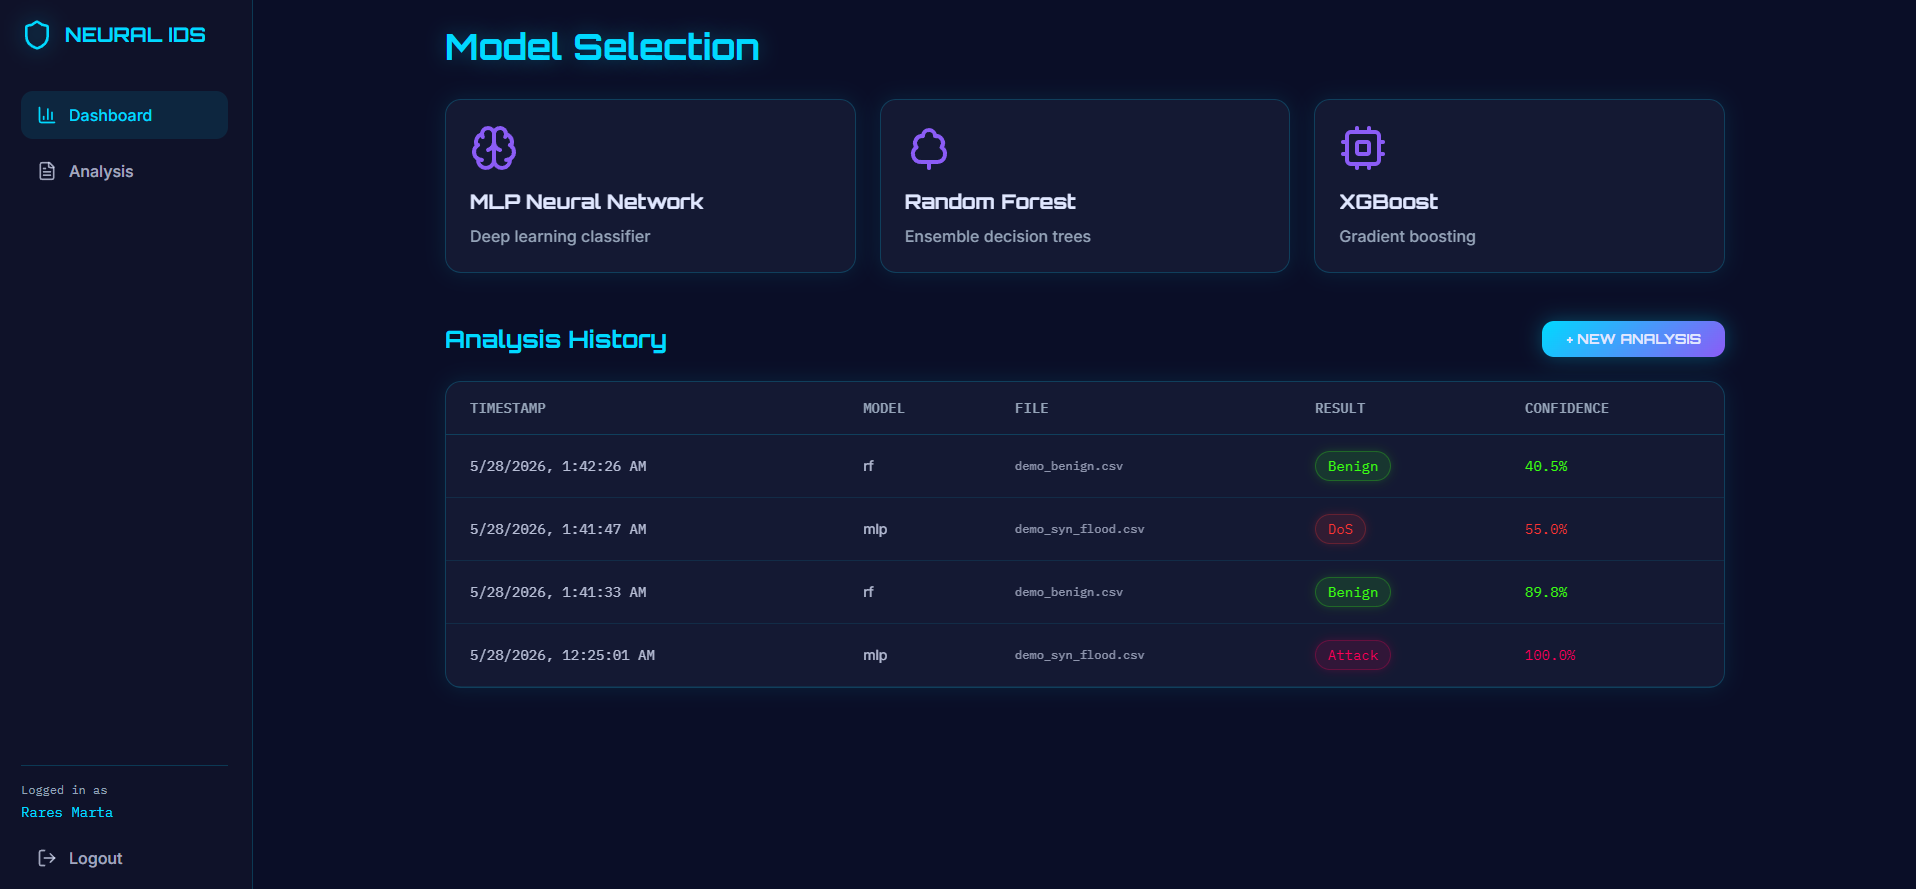
\includegraphics[width=0.82\textwidth]{figures/app_dashboard.png}
    \caption{The NEURAL IDS landing screen, which introduces the system and leads into the dashboard for model selection, upload, and the session's analysis history.}
    \label{fig:app_dashboard}
\end{figure}

\begin{figure}[htbp]
    \centering
    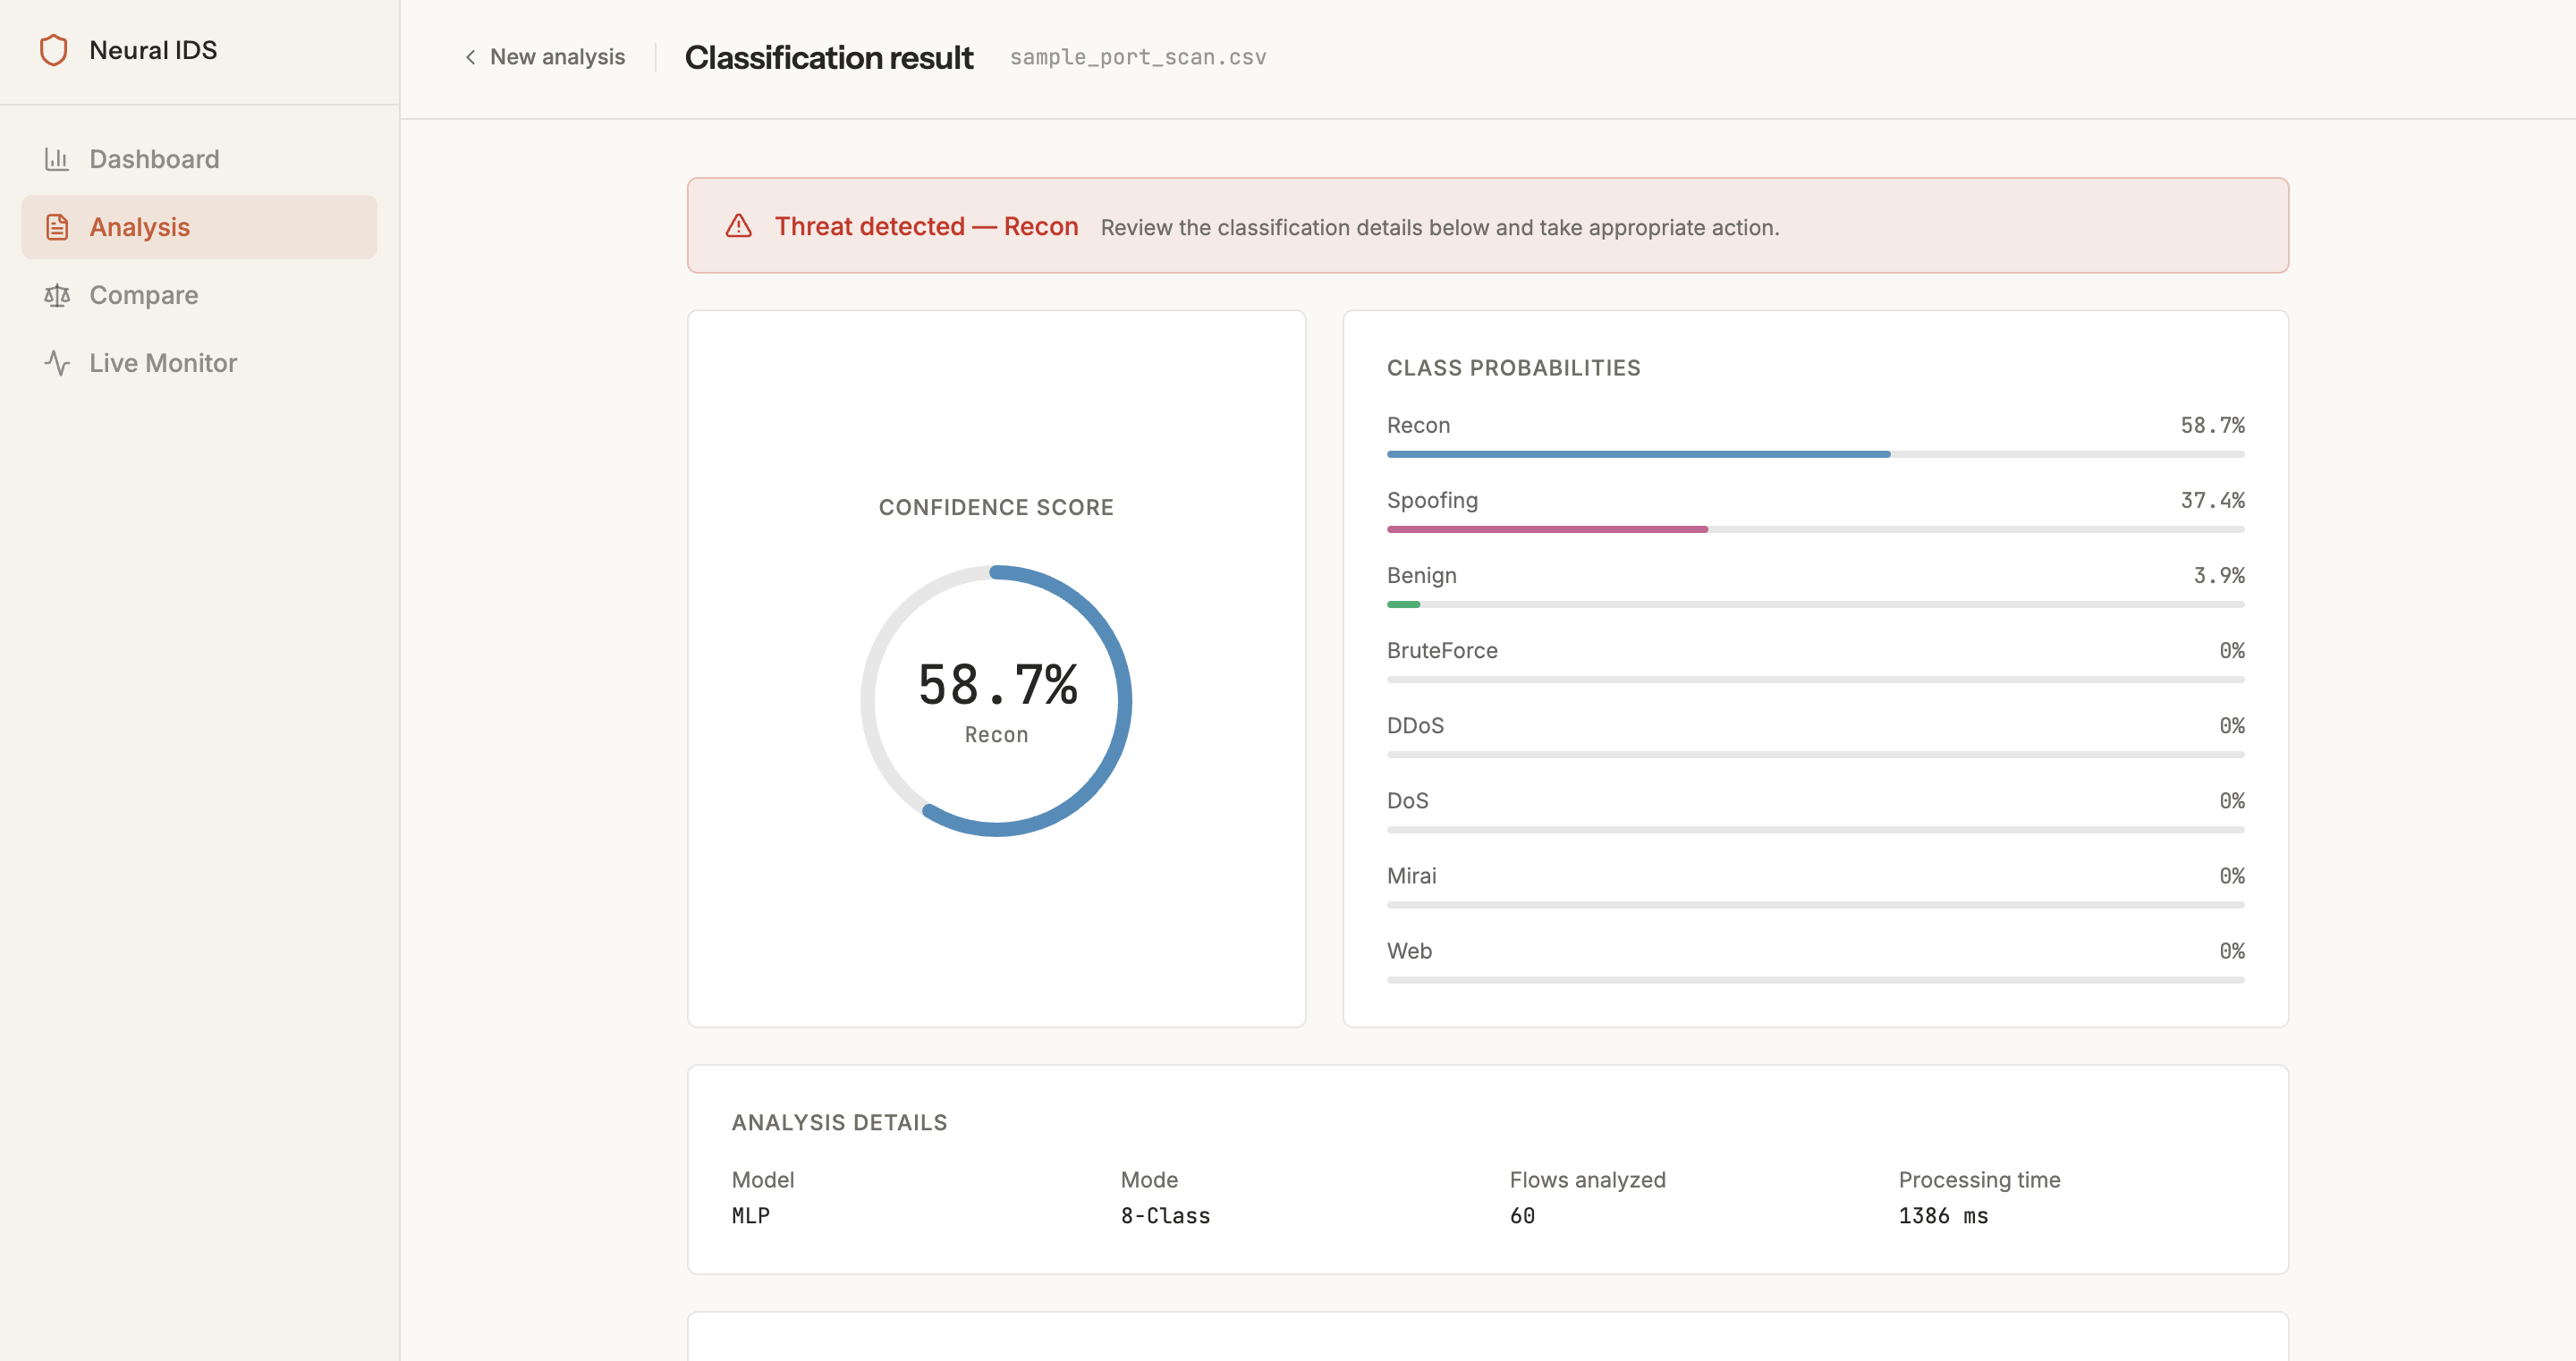
\includegraphics[width=0.95\textwidth]{figures/app_attack.png}
    \caption{A classification result in NEURAL IDS: a port-scan capture classified at the 8-class granularity as \textbf{Recon} (reconnaissance), the correct family for scanning traffic, with Spoofing second. The screen shows the confidence gauge, the ranked class probabilities, and the run metadata. The processing time shown includes the on-demand SHAP explanation (the local feature attribution of Section~\ref{subsec:xai_ids}), so it is larger than the raw inference latency benchmarked in Chapter~\ref{chap:results} (NFR-1).}
    \label{fig:app_attack}
\end{figure}

\subsection{Authentication, Persistence, and Deployment}
\label{subsec:auth_persistence}

\par Because the demo is public, each user's history has to stay private, so the frontend talks to two independent backends (Figure~\ref{fig:deployment_topology}). The first is the \emph{stateless inference channel}: the React app sends a cross-origin \texttt{POST /api/classify} to the FastAPI backend on Hugging Face Spaces and gets back a JSON verdict; that backend holds no database and remembers nothing between requests. The second is the \emph{stateful identity-and-history channel}: the same app talks to a managed Supabase project for sign-in and for storing past results. The two never share server-side state, so either can be replaced without touching the other and an inference request never waits on the database.

\par Supabase is used because it bundles managed email/password authentication with a Postgres database and row-level security, which avoids building a separate auth service. On sign-in the client receives a JSON Web Token, attaches it to later requests, and restores the session from the stored token on reload. After each classification the result screen writes one row to the \texttt{analyses} table, tagged with the user's identifier: a UUID key, the \texttt{user\_id}, a server timestamp, the variant and granularity, the input type, the file name, the top label with its calibrated confidence, and the full probability vector as JSON. The uploaded traffic itself is never stored, only this derived metadata, which keeps the table consistent with FR-D5. Privacy does not depend on the client: a row-level-security policy limits every read and write to rows whose \texttt{user\_id} matches the caller, so one user can never see another's history even though all rows live in one table.

\par For deployment the backend is packaged as a Docker image on Hugging Face Spaces and the frontend is served from Vercel, so the demo works from any browser without the presenter's laptop being reachable. For the local defence the same backend runs on the laptop over loopback, with the frontend served from the same machine. Figure~\ref{fig:deployment_topology} shows the result: Vercel serves the static application, which at runtime fans out to the two independent backends.

\begin{figure}[htbp]
    \centering
    \resizebox{0.72\textwidth}{!}{%
    \begin{tikzpicture}[
        node distance=1.8cm and 2.2cm,
        box/.style={
            rectangle, rounded corners=4pt, draw=black!70, thick,
            minimum width=3.2cm, minimum height=1.4cm, text width=3.4cm,
            align=center, font=\small
        },
        client/.style={box, fill=gray!12},
        edge/.style={box, fill=gray!6},
        infer/.style={box, fill=green!10},
        store/.style={box, fill=yellow!20},
        arrow/.style={->, >=latex, thick, black!65},
        biarrow/.style={<->, >=latex, thick, black!65},
        lbl/.style={font=\scriptsize, black!60, align=center}
    ]
    % Client (top)
    \node[client] (browser) {\textbf{Client browser}\\[2pt] NEURAL IDS\\ React SPA};

    % Infrastructure row (bottom)
    \node[infer, below=of browser]      (hf)     {\textbf{Hugging Face Spaces}\\[2pt] Docker container\\ FastAPI \texttt{/api/classify}\\ + model artefacts};
    \node[edge, left=of hf]             (vercel) {\textbf{Vercel}\\[2pt] static CDN\\ serves the built\\ React SPA};
    \node[store, right=of hf]           (supa)   {\textbf{Supabase}\\[2pt] Auth (JWT)\\ Postgres \texttt{analyses}\\ row-level security};

    % Delivery of the SPA
    \draw[arrow] (vercel.north) to[out=90, in=180]
        node[lbl, above left, pos=0.6] {HTTPS\\ app bundle} (browser.west);

    % Stateless inference channel
    \draw[biarrow] (browser.south) -- node[lbl, right] {HTTPS \texttt{POST}\\ \texttt{/api/classify} (CORS)\\ $\rightarrow$ JSON verdict} (hf.north);

    % Stateful identity + history channel
    \draw[biarrow] (browser.east) to[out=0, in=90]
        node[lbl, above right, pos=0.4] {HTTPS\\ auth + history\\ insert / select} (supa.north);

    % Channel annotations
    \node[lbl, below=0.15cm of hf, green!45!black] {\itshape stateless inference channel};
    \node[lbl, below=0.15cm of supa, orange!60!black] {\itshape stateful identity \& history channel};

    \end{tikzpicture}%
    }
    \caption{Runtime deployment topology. Vercel delivers the static React SPA (grey); at runtime the SPA drives two independent backends -- a \emph{stateless} inference service on Hugging Face Spaces (green), reached via \texttt{POST /api/classify}, and a \emph{stateful} Supabase project (yellow) for authentication and per-user history. The two channels share no server-side state, so inference never blocks on persistence and either tier can be replaced in isolation.}
    \label{fig:deployment_topology}
\end{figure}

\section{Implementation Notes}
\label{sec:implementation_details}

\par A few choices turn this design into working code. The offline pipeline stays within a modest memory budget by reading raw CSVs lazily and only materialising after columns are projected; the deduplicated, subsampled frame is the only large object held, and it is freed once converted to arrays. Reproducibility comes from broadcasting one seed to every random source -- the numerical library, the deep-learning framework on CPU and GPU, its deterministic flags, and the samplers -- so re-running on the same files reproduces the metrics to within a few thousandths of an F1 point. All the constants (the per-class cap, the 25-feature selection, the active splits and granularities, the batch size, the epoch and early-stopping settings, the learning rate, and the seed) live in one configuration module shared by the notebook and the headless training command, so the two can never disagree. The runtime needs only the standard scientific-Python stack plus a lightweight web framework: there is no separate serving framework (the model is loaded straight into the application process) and no packaging beyond a single directory launched by one command, which satisfies NFR-4.

\section{Testing Strategy}
\label{sec:testing_strategy}

\par The application is tested at three levels: sanity checks inside the training pipeline, an artefact round-trip test per variant, and an end-to-end functional acceptance test.

\subsection{Pipeline Sanity Checks}
\label{subsec:notebook_sanity}

\par The pipeline asserts and prints checks at each step. One assertion confirms the fine-grained label map covers every attack folder exactly once; another confirms ingestion leaves no folder unmapped, so a newly added attack folder cannot be silently dropped. For each split it checks that every fine-grained label appears at least once in the training partition and warns if not. Per-folder row counts (raw, deduplicated, sampled) are printed, so a sudden change in the source data shows up immediately.

\subsection{Artefact Round-Trip Test}
\label{subsec:roundtrip_test}

\par For every variant, after training, the pipeline reloads the freshly written files through the exact code path the demo uses and predicts on the test partition, then checks those predictions match the still-in-memory model's exactly. This caught two real bugs during development: a column-ordering drift between training and inference, and a silent dtype mismatch when arrays became tensors without an explicit precision cast.

\subsection{Functional Acceptance Test}
\label{subsec:f1_functional_test}

\par The core function is checked end-to-end on two inputs whose correct labels are known in advance, so each run either clears a fixed threshold or it does not. The benign baseline is a short capture of normal browsing made on the demo machine; it passes if at least 95\% of flows are predicted Benign at the binary granularity. The flood is a SYN-flood capture against a local target made with a standard packet-crafting tool; it passes if at least 95\% of flows are predicted Attack at the binary granularity and the dominant family at the 8-class granularity is a denial-of-service family. These thresholds sit well below the test-set numbers, so the test tolerates the shift between the training data and the demo machine while still failing loudly if the demo is wired to the wrong scaler or encoder.

\subsection{Negative-Path Testing}
\label{subsec:negative_path_testing}

\par Three failure cases are exercised manually, since they reproduce from a brief interactive session. A CSV missing one or more expected feature columns produces a domain error naming the missing columns (FR-D4). A non-capture file (for example a text file renamed to a capture extension) produces a flow-extraction error carrying the tool's own stderr (also FR-D4). Starting the demo with no artefacts on disk exits quickly with a message pointing back to the training pipeline (FR-D2).

\section{Functional Acceptance Evidence}
\label{sec:f1_acceptance_evidence}

\par The acceptance test of Section~\ref{subsec:f1_functional_test} was run against the deployed system through the NEURAL IDS frontend, using two pre-extracted CSVs with known labels: \texttt{sample\_benign\_browsing.csv} (normal browsing) and \texttt{sample\_syn\_flood.csv} (a SYN flood against a local target). Both passed. For the SYN flood, the binary MLP labelled every flow Attack (mean calibrated confidence 99.6\%) and the 8-class variant confirmed DoS as the dominant family -- both correct. For the benign capture, the binary MLP returned Benign on 98\% of flows, above the 95\% threshold, discharging the no-false-alarm half of the test. (Confidence here is the mean softmax probability of the dominant class after temperature scaling, not the share of flows in that class.)

\par Figure~\ref{fig:app_attack} shows the result screen on a third capture, a port scan: the 8-class MLP labels it Recon, the reconnaissance family, which is the expected result for scanning traffic. Together the runs show the end-to-end path working -- upload, flow features, prediction, and a calibrated verdict -- across benign, denial-of-service, and reconnaissance traffic.
